\documentclass{article}
\usepackage{geometry}[a4paper, margin=1in]
\usepackage{graphicx}
\usepackage{float}
\usepackage{subfigure}
\title{Practical Submission Sheet}
\newcommand{\bb}[1]{\textbf{#1}}
\date{}
\begin{document}
	\maketitle
	\begin{tabular}{ll}
		\bb{Term}: 2020-1 & \bb{Submission Date}: August 28th, 2020.\\
		\bb{Lecture Date}: August 28th, 2020. & \bb{Practical Number}: 4\\
		\bb{Course Code}: PHY249 & \bb{Section}: G2903\\
		\bb{Registration Number}: 11912610 & \bb{Roll No}: 03\\
		\bb{Student Name}: Aayush Arya & \\
	\end{tabular}
	
	\section*{Concepts Learnt}
	Learnt different types of logic gates, how a single \textit{unviversal} can be used to create other gates, how deMorgan's theorem helps us understand logic using boolean algebra.
	
	\section*{Key Observations \& Insights}
	The use of the NAND gate to replicate the behavior of other gates, namely AND and OR was tested. The effect of a zener diode in a circuit for current stabilization was tested. \\Physically, logic gates in essence are nothing but transistor circuits.
	
	\section*{Application Areas}
	The existence of a 
	\textit{universal} gate means that if we have a discrete or integrated device with only type of gate, any other desired logical can be obtained.\\Zener diodes are useful in situations when a constant voltage supply is to be maintained.

	\section*{Report}
	NAND and NOR gates are known to be \textit{universal} gates \textemdash any other type of logic gate can be constructed by combining units of NAND or NOR alone. Here, we simulate the such a construction for the case of AND and OR gates.
	\begin{figure}[H]
		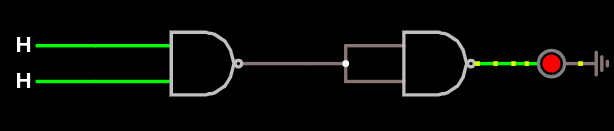
\includegraphics[width=\textwidth]{AND.png}
		\caption{Circuit equivalent to an AND gate using just NAND gates.}
	\end{figure}
	For making an AND gate, we need a method to invert the output of a NAND gate. If we take another NAND gate and short circuit its input terminals, it behaves at a NOT gate/inverter. The reason being, it now takes only one input for both the terminals combined (both inputs would be either 0 or 1). When 0 is input to this, the NAND output would be 1 and in the case when 1 is input, this gate gives 0.\\
	
	 An AND gate is thus constructed as shown in figure 1.
	\begin{figure}[H]
		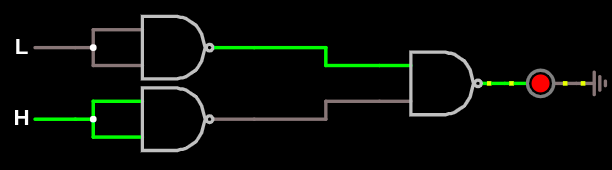
\includegraphics[width=\textwidth]{OR.png}
		\caption{An equivalent OR gate created using NAND gates.}
	\end{figure}

An analogous combination of NAND gates to construct an OR gate was also used, as shown in Figure 2.
	\begin{figure}[H]
		\centering
		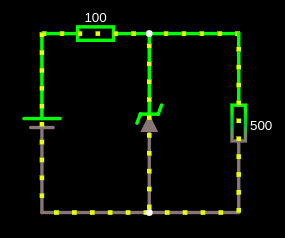
\includegraphics{zener_circuit}
		\caption{Zener circuit}
	\end{figure}
A zener diode behaves as an emf source. When a load resistance is applied across two voltage supplies in parallel, the $V_0$ across it is controlled solely by the source right next to it. Therefore, a zener diode can be effectively used a voltage stabilizer.
\end{document}